\documentclass[11pt, a4paper]{article}
\usepackage{fullpage}
\usepackage{mathtools}
\usepackage{chemfig}
\usepackage{pdfpages}

\begin{document}

\title{ALC Tagesbericht\\ vom 15.01.19}
\author{Janosch Ehlers, Jacqueline Preis}
\maketitle

	\begin{center}
	\textsc{Elektrochemische Experimente}
	\end{center}

\section{10.1 Chemischer Eisen-Eintopf}

In diesem Versuch werden nacheinander verschiedene Lösungen zusammen gegeben, wodurch sich verschiedene Stoffe und Komplexe bilden. 

\textsc{Versuchsdurchführung:} Siehe Skript.\\

\textsc{Beobachtung:}\hspace{5mm} Die Beobachtungen sind in der Folgenden Tabelle aufgeführt:\\

\begin{center}
\textsc{Tabelle 1: Beobachtungen Versuch 10.1}\\
\begin{tabular}{cc}
Zugabe von.. & Beobachtung\\
\hline
Natriumcitrat & Schwach gelb\\
Natronlauge & Über grün zu dunkelblau, trüb\\
Wasserstoffperoxid (3\%) & Dunkelgrün/braun\\
Salzsäure & Dunkelrot\\
Natriumsalicylat & Dunkelrot bis schwarz\\
Schwefelsäure & Dunkelrot bis schwarz\\
Kaliumthiocyanat & Dunkelrot\\
Zinn(II)chlorid & Dunkelrot\\
Kaliumhexacyanoferrat & Dunkelblau \\
Wasserstoffperoxid (3\%) & Schwarz\\
Natronlauge & Dunkelbraun\\
Natriumsulfid & Dunkelgrün bis schwarz\\
\end{tabular}
\end{center}

\textsc{Auswertung:}\hspace{8mm} Folgende Reaktionsgleichungen waren bei diesem Versuch beteiligt:\\
\begin{enumerate}
\item $Fe^{2+}_{(aq)} + C_5H_6O^{3-}_{7(aq)} \rightleftharpoons Fe(C_5H_6O_7)^-$
\item $Fe(C_5H_6O_7)^- + 2\cdot OH^-_{(aq)} \rightleftharpoons Fe(OH)_2 + C_5H_6O^{3-}_{7(aq)}$
\item $2\cdot Fe(OH)_2 + H_2O_2 \rightleftharpoons 2\cdot Fe(OH)_3$
\item $Fe(OH)_3 + 3\cdot H^+_{(aq)} + 4Cl^-_{(aq)}  \rightleftharpoons FeCl^-_{4(aq)} + 3\cdot H_2O$
\item $FeCl^-_{4(aq)} + C_7H_5O^-_{3(aq)} \rightleftharpoons Fe(C_7H_5O_3)^{2+}_{(aq)} + 4\cdot Cl^-_{(aq)}$
\item $Fe(C_7H_5O_3)^{2+}_{(aq)} + H^+_{(aq)} \rightleftharpoons Fe^{3+} + C_7H_5O^{3-}_{(aq)}$
\item $Fe^{3+}_{(aq)} + SCN^-_{(aq)} \rightleftharpoons Fe(SCN)^{2+}_{(aq)}$
\item $2\cdot Fe(SCN)^{2+}_{(aq)} + Sn^{2+}_{(aq)} \rightleftharpoons 2\cdot Fe^{2+}_{(aq)} + Sn^{4+}_{(aq)} + 2\cdot SCN^-_{(aq)}$
\item $2\cdot Fe^{2+}_{(aq)} + Fe(CN)^{4-}_{6 (aq)} \rightleftharpoons Fe_2[Fe(CN)_6]_{(aq)}$                                              
\item $2\cdot Fe^{2+}_{(aq)} + \frac{1}{2}H_2O_2 + H^+_{(aq)} \rightleftharpoons 2\cdot Fe^{3+}_{(aq)} + H_2O$
\item $Fe^{3+}_{(aq)} + 3\cdot OH^-_{(aq)} \rightleftharpoons Fe(OH)_3$
\item $2\cdot Fe(OH)_3 + 3\cdot S^{2-}_{(aq)} \rightleftharpoons 2\cdot FeS + S + 6\cdot OH^-_{(aq)} $
\end{enumerate}
Die wichtigsten Strukturformeln für diese Reaktion sind:\\

Zitronensäure ($C_6H_5O_3$):\\
$$\chemfig{HO-[1](=[2]O)-[7]-[1](-[2](=[3]O)-[1]OH)(-[6]OH)-[7]-[1](=[2]O)-[7]OH}$$ \\ %Zitronensäure

Salicylsäure ($C_7H_6O_2$):\\
$$\chemfig{**6(---(-OH)-(-[2](=[3]O)-[1]OH)--)}$$\\ %Benzen

Hexacyanoferrat ($Fe(CN)_6$):\\
$$\left[\chemfig{Fe(-[:30]C~[:30]N)(-[:90]C~[:90]N)(-[:150]C~[:150]N)(-[:210]C~[:210]N)(-[:270]C~[:270]N)(-[:330]C~[:330]N)}\right]^{4-}$$\\ %Hexacyanoferrat

\section{10.2 Ioduhr}

Dieser Versuch zeigt die Abhängigkeit der Reaktionsgeschwindigkeit von der Konzentration am Beispiel der Ioduhr. 

\textsc{Versuchsdurchführung:} Siehe Skript.\\

\textsc{Beobachtung:}\hspace{5mm} Die Angangskonzentrationen von Iodat und Sulfat sowie die Reaktionszeit wird dem Versuchsansatz in der Folgenden Tabelle Zugeordnet: \\
\begin{center}
\textsc{Tabelle 2: Messergebnisse Versuch 10.2}\\
\begin{tabular}{cccc}
Ansatz & [Iodat] & [Sulfit] & $\text{Reaktionszeit}_{[s]}$\\
\hline
1 & 4,8 & 2,19 & 18\\
2 & 3,2 & 1,48 & 53\\
3 & 2,4 & 1,1 & 119\\
\end{tabular}
\end{center}

\begin{flushleft}

\textsc{Auswertung:}\hspace{8mm} Es handelt sich um eine Reaktion 1. Ordnung. Für Reaktionen 1. Ordnung gilt: Je höher die Edukt-Konzentration, desto schneller läuft die Reaktion ab (vgl. Skript S. 105f.). Dies spiegelt sich in den Versuchsergebnissen\\ wider; in Ansatz 1 ist die höchste Konzentration an Iodat
(vgl. Tabelle 2) und die Reaktion läuft am schnellsten ab, wohingegen Ansatz 3 die niedrigste Konzentration aufweist und die Reaktion am langsamsten abläuft (vgl. Tabelle 2). 
Normalerweise sollte die Verdoppelung der Konzentration auch eine Steigerung der Reaktionsgeschwindigkeit ergeben (vgl. Skript S. 108).  Dies war in unserer Versuchsdurchführung jedoch nicht der Fall.\\ Während  sich die Konzentration von Ansatz 3 zu Ansatz 1 verdoppelt von 2,4 mmol/l auf 4,8 mmol/l, steigert sich die Reaktionsgeschwindigkeit etwa um den Faktor 6, und zwar von 119 Sekunden zu 18 Sekunden. 
Eine Fehlerquelle könnte das ungleichmäßige Rühren sein, da das Rühren die Wahrscheinlichkeit, dass zwei Teilchen aufeinanderstoßen und miteinander reagieren, erhöht, und somit die Reaktionsgeschwindigkeit steigert.
\end{flushleft}

\newpage
\section{10.3 T-Abhängigkeit der Reaktionsgeschwindigkeit}


\begin{center}
\textsc{Teilversuch A}
\end{center}
\textsc{Versuchsdurchführung:} Siehe Skript.\\

\textsc{Beobachtung:}\hspace{5mm} Die Messwerte dieses Versuchs können der Tabelle 1 entnommen werden.\\
\begin{center}
\textsc{Tabelle 1:}\\
\begin{tabular}{cc}
Temperatur & Zeit\\
\hline
$19,4^\circ C$ & 10 Min\\
$2^\circ C$ & 0:51,6 Min\\
$-11^\circ C$ & 6:02 Min\\
\end{tabular}
\end{center}

\textsc{Auswertung:}\hspace{8mm} Bei diesem Versuch liegt eine Redoxreaktion vor:\\
\begin{center}
\begin{tabular}{crcl}
Ox: & $Mg^0$ & $\rightleftharpoons$ & $Mg^{2+}+2e^-$\\
Red: & $H_2^{+I}SO_4 + 2e^-$ & $\rightleftharpoons$ & $H_2^0 + SO_4^{-2}$\\
\hline
 & $Mg_{(s)} + H_2SO_{4(aq)}$ & $\rightleftharpoons$ & $H_{2}\uparrow_{(g)} + MgSO_4$\\
\end{tabular}
\end{center}
\vspace{5mm}
\begin{center}
\textsc{Teilversuch B}
\end{center}

\textsc{Versuchsdurchführung:} Siehe Skript.\\

\textsc{Beobachtung:}\hspace{5mm} Die Messwerte dieses Versuchs können der Tabelle 1 entnommen werden.\\
\begin{center}
\textsc{Tabelle 1:}\\
\begin{tabular}{cc}
Temperatur & Zeit\\
\hline
$-19,1^\circ C$ & 2:41 Min\\
$-0,3^\circ C$ & 1:50 Min\\
$19,4^\circ C$ & 0:47 Min\\
\end{tabular}
\end{center}

\textsc{Auswertung:}\hspace{8mm} Die hier zugrundeliegende Reaktionsgleichung ist im folgenden beschrieben:
\begin{center}
\begin{tabular}{crcl}
Ox: & $Zn^0$ & $\rightleftharpoons$ & $Zn^{2+}+2e^-$\\
Red: & $H_2^{+I}SO_4 + 2e^-$ & $\rightleftharpoons$ & $H_2^0 + SO_4^{-2}$\\
\hline
 & $Zn_{(s)} + H_2SO_{4(aq)}$ & $\stackrel{CuSO_4}{\rightleftharpoons}$ & $H_{2}\uparrow_{(g)} + ZnSO_4$\\
\end{tabular}
\end{center}
Ein Diagramm, welches den Natürlichen Logarithmus der Zeit über dem Rezipropwert der Temperatur darstellt, ist im Anhang unter Diagramm 5 zu finden. Hier sieht man deutlich das sich die Messwerte innerhalb einer verhältnismäßig geringen Abweichung auf einer Linie anordnen.
\newpage
\section{4.4 Hydrolyse von tert-Butylchlorid}

\textsc{Versuchsdurchführung:} Siehe Skript.\\

\textsc{Beobachtung:}\hspace{5mm} Unsere Messergebnisse können der folgenden Tabelle entnommen werden:\\
\begin{center}
\textsc{Tabelle 3: Messergebnisse und Berechnungsergebnisse von Versuch 10.4}\\
\begin{tabular}{cccc}
$Zeit_{[s]}$ & $\textrm{Stromstärke}_{[\mu A]}$ & $\ln([a])$\\
\hline
$0$ & $0$ & $--$\\
$15$ & $195$ & $-8,65$\\
$30$ & $208,9$ & $-8,7$\\
$45$ & $210$ & $-8,8$\\
$60$ & $211,1$ & $-8,91$\\
$75$ & $210,3$ & $-9,02$\\
$90$ & $212,5$ & $-9,13$\\
$105$ & $211,1$ & $-9,24$\\
$120$ & $212,7$ & $-9,35$\\
$135$ & $212,2$ & $-9,46$\\
$150$ & $212$ & $-9,57$\\
$165$ & $212,8$ & $-9,68$\\
$180$ & $212$ & $-9,8$\\
$195$ & $212,1$ & $-9,91$\\
$210$ & $213,2$ & $-10,01$\\
$225$ & $212,7$ & $-10,13$\\
$240$ & $212$ & $-10,24$\\
$255$ & $213,7$ & $-10,35$\\
$270$ & $212$ & $-10,47$\\
$285$ & $213,7$ & $-10,57$\\
$300$ & $212,6$ & $-10,69$\\
$315$ & $212$ & $-10,8$\\
$330$ & $213$ & $-10,91$\\
$345$ & $213,2$ & $-11,02$\\
$360$ & $212,2$ & $-11,13$\\

\end{tabular}
\end{center}

\textsc{Auswertung:}\hspace{8mm} Die Diagramme, in denen die einzelnen Größen über die Zeit aufgetragen sind, sind im Anhang einsehbar. Bei dieser Reaktion ist die Größe Ln([A]) von Bedeutung. Aus ihrem Verlauf kann in diesem Fall bestimmt werden, um welche Ordnung es sich hier handelt. Es wurde die These aufgestellt, dass es sich hier um eine Reaktion 1. Ordnung handelt. Der funktionelle Zusammenhang von Konzentration und Anfangskonzentration des Stoffes ist über $$[A] = [A]_0 \cdot e^{-kt}$$ definiert. Die Anfangskonzentration ist hier gleichzusetzen mit der größten gemessenen Stromstärke, da $[(CH_3)_3CCl]_0 = [H^+]_\infty\sim LF_\infty \sim I_\infty$. Allerdings muss beachtet werden das bei einer Gleichsetzung sowohl die Proportionalitätskonstante als auch die Verschiebungskonstante fehlt. Wodurch unser Ergebnis nun eher qualitativ ist, als quantitativ ist. Für das Auftragen von Konzentration über die Zeit muss nun die Proportionalitätskonstante k ermittelt werden. Diese ist näherungsweise aus den Messergebnissen zu entnehmen. Dabei tragen wir $$\ln\left(1-\frac{I}{I_\infty}\right)$$ gegen die Zeit auf und ermittel die Steigung der Trendgeraden. Diese ist in meinem Fall: $k=-0,00743357230937$(siehe Diagramm 6) dieser Wert kann nun für das Errechnen der Konzentration nach $$[A] = [A]_0\cdot e^{-kt}$$ verwendet werden. Die Werte aus dieser Zuordnung in Abhängigkeit der Zeit können der Diagramm 4 entnommen werden. Für den Versuch interessant, ist allerdings der Logarithmus der eben berechneten Werte. Diese sind in Diagramm 3 dargestellt.Aus dem Verlauf der annähernden Geraden ist zu erkennen, dass diese Reaktion somit eine Reaktion erster Ordnung ist.\\ 
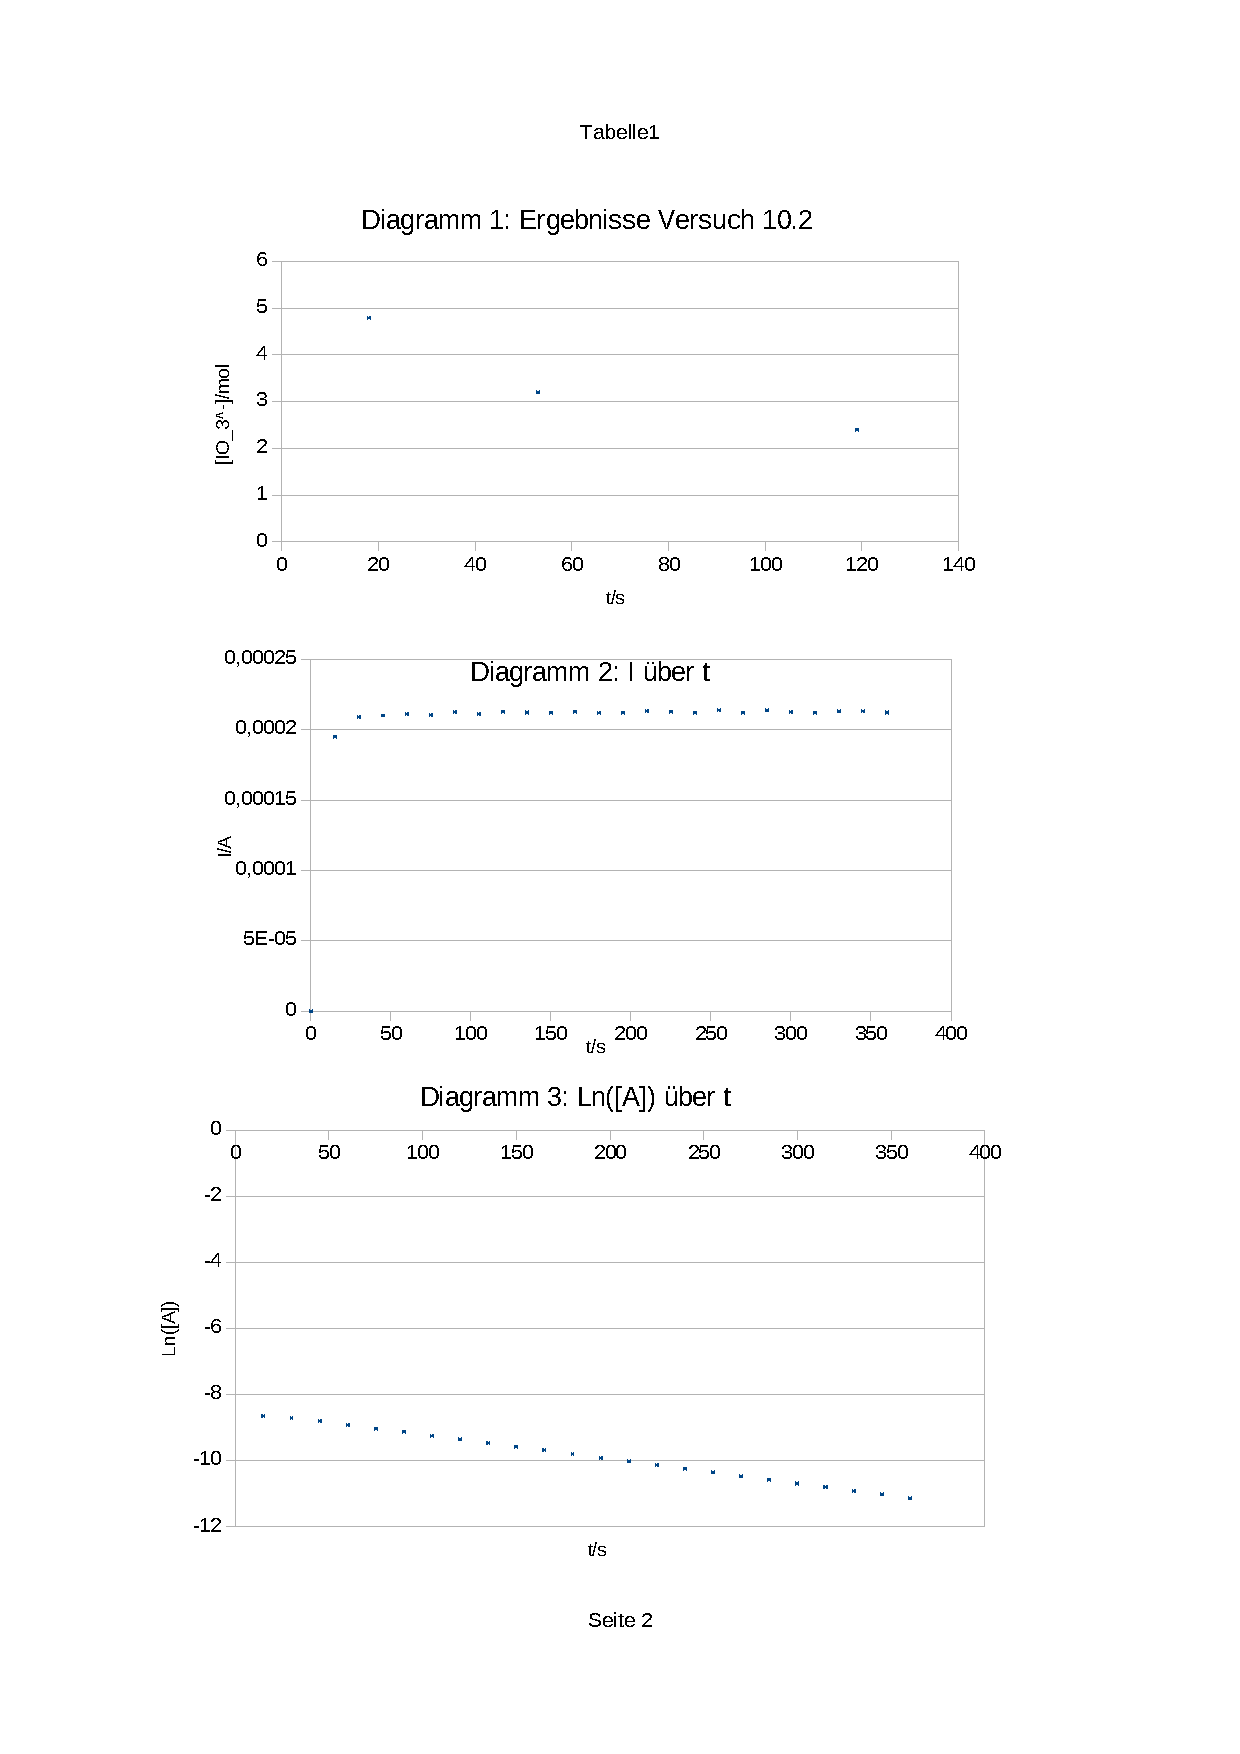
\includepdf[pages=1]{./Diagramme.pdf}
\includepdf[pages=2]{./Diagramme.pdf}

\end{document}